% Section 2: Mathematical Foundations
\section{Mathematical Foundations}
\label{sec:math}

\subsection{Clifford Algebra Cl(3,1)}

The foundation of our approach lies in the Clifford algebra $\Cl(3,1)$, which provides the natural algebraic framework for describing spinors and the geometry of spacetime.

\begin{definition}[Clifford Algebra]
The Clifford algebra $\Cl(3,1)$ is the associative algebra over $\mathbb{R}$ generated by $\{\gamma^0, \gamma^1, \gamma^2, \gamma^3\}$ with relations:
\begin{equation}
    \{\gamma^\mu, \gamma^\nu\} = 2\eta^{\mu\nu} \mathbf{1}
\end{equation}
where $\eta^{\mu\nu} = \diag(-1, 1, 1, 1)$ is the Minkowski metric.
\end{definition}

The algebra has dimension $2^4 = 16$ and decomposes as:
\begin{equation}
    \Cl(3,1) \cong \text{Mat}(4, \mathbb{R})
\end{equation}

A basis is given by:
\begin{align}
    &\{1\} && \text{(1 scalar)} \\
    &\{\gamma^\mu\} && \text{(4 vectors)} \\
    &\{\gamma^{\mu\nu} = \gamma^{[\mu}\gamma^{\nu]}\} && \text{(6 bivectors)} \\
    &\{\gamma^{\mu\nu\rho} = \gamma^{[\mu}\gamma^\nu\gamma^{\rho]}\} && \text{(4 trivectors)} \\
    &\{\gamma^{0123} = \gamma_5\} && \text{(1 pseudoscalar)}
\end{align}

\subsection{Spin Group and Covering Maps}

The spin group $\Spin(3,1)$ is the double cover of the proper orthochronous Lorentz group $SO^+(3,1)$:
\begin{equation}
    \rho: \Spin(3,1) \to SO^+(3,1)
\end{equation}

with kernel $\ker(\rho) = \{+1, -1\} = Z_2$.

\begin{theorem}[Universal Covering]
The map $\rho$ is a universal covering homomorphism, making $\Spin(3,1)$ the universal covering group of $SO^+(3,1)$.
\end{theorem}

\subsection{Spectral Dimension}

The spectral dimension provides an effective notion of dimension that can vary with energy scale.

\begin{definition}[Spectral Dimension]
For a Riemannian manifold $(M, g)$, the spectral dimension is defined through the heat kernel trace:
\begin{equation}
    Z(t) = \Tr(e^{t\Delta})
\end{equation}
where $\Delta$ is the Laplace-Beltrami operator. The spectral dimension at scale $\ell = \sqrt{t}$ is:
\begin{equation}
    \ds(\ell) = -2 \frac{d \ln Z(t)}{d \ln t}
\end{equation}
\end{definition}

In our framework, the spectral dimension runs from $\ds = 10$ at the Planck scale to $\ds = 4$ at macroscopic scales:
\begin{equation}
    \ds(T) = 4 + \frac{6}{1 + (T/T_c)^2}
\end{equation}
where $T_c \sim 10^{16}$ GeV is the GUT scale.

\begin{figure}[htbp]
\centering
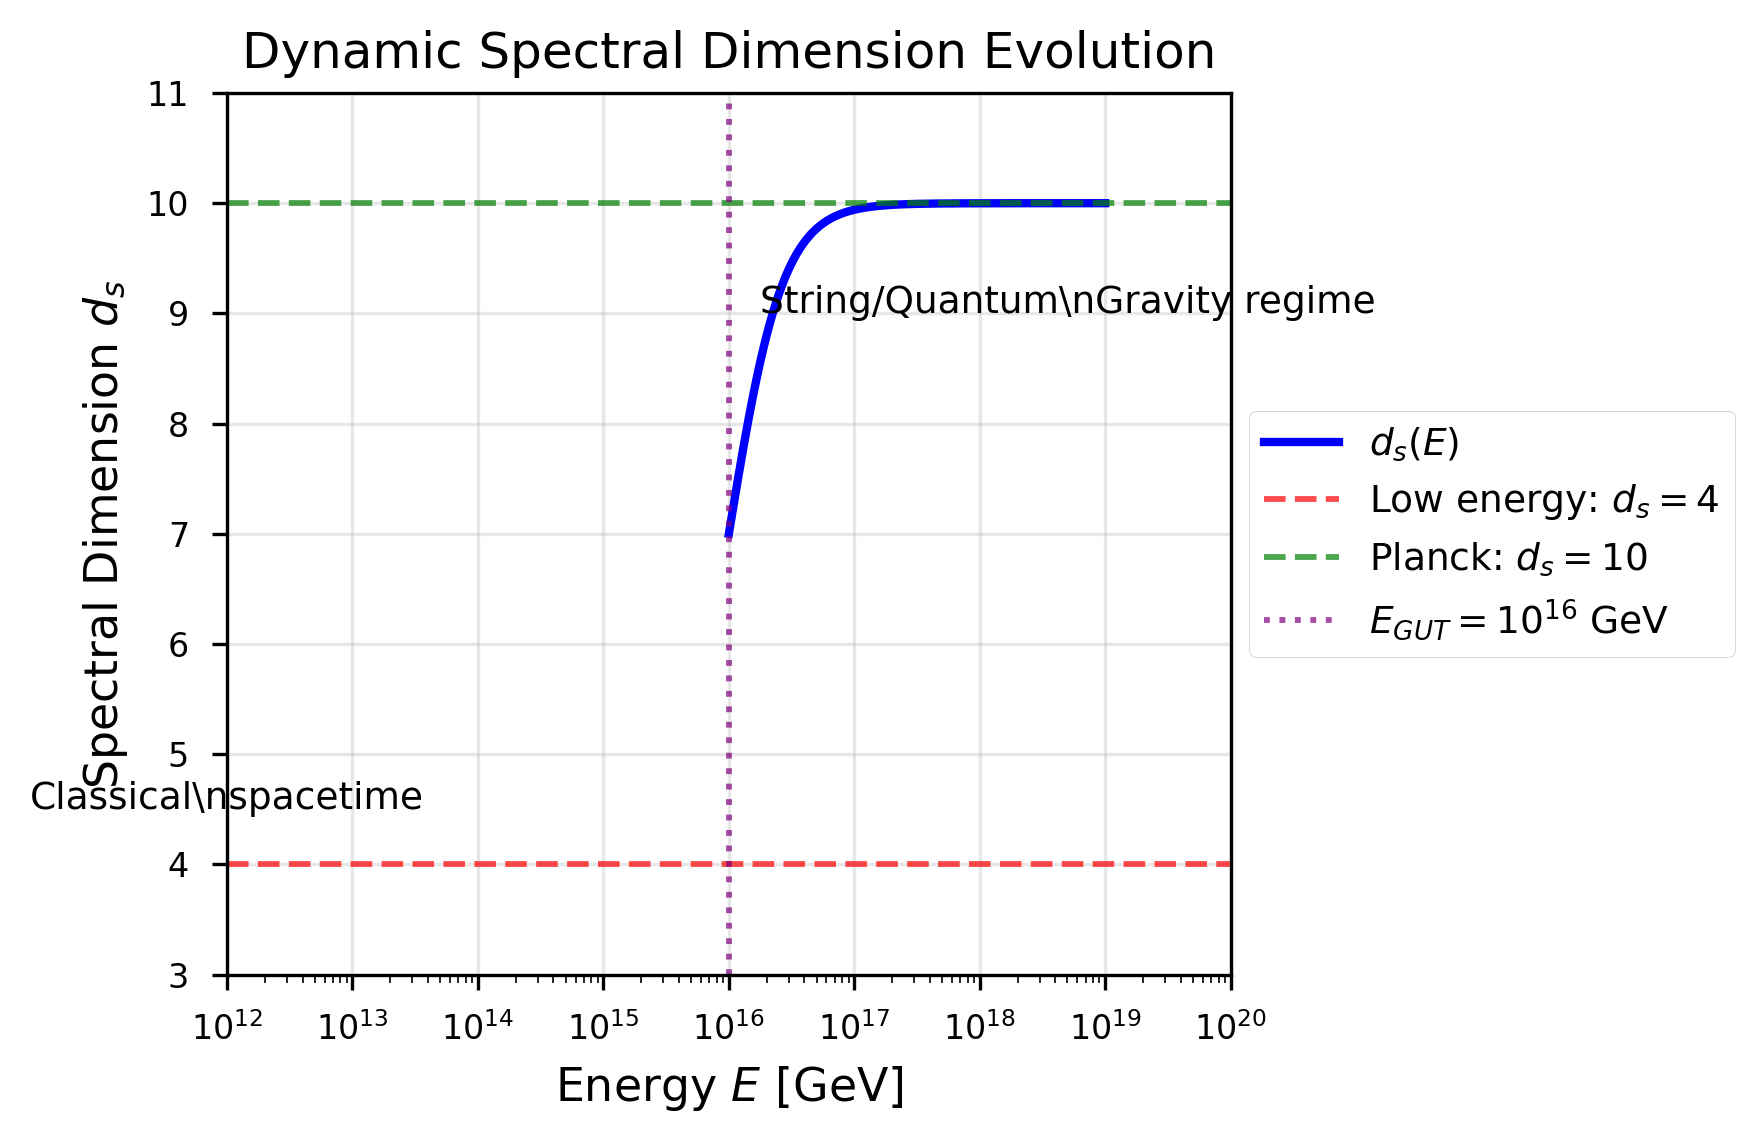
\includegraphics[width=0.8\textwidth]{figures/fig1_spectral_dimension.png}
\caption{Dynamic spectral dimension evolution. At high energies ($E \gg E_{GUT}$), the spectral dimension approaches 10, while at low energies it freezes to 4.}
\label{fig:spectral_dimension}
\end{figure}

\subsection{Fractal Measures}

The Hausdorff dimension $d_H$ and spectral dimension $\ds$ characterize the fractal structure of spacetime at small scales.

\begin{definition}[Fractal Measure]
The fractal measure on a set $S$ is defined by:
\begin{equation}
    \mu_\alpha(S) = \lim_{\delta \to 0} \inf \left\{\sum_i (\text{diam } U_i)^\alpha : S \subseteq \bigcup_i U_i, \text{diam } U_i < \delta\right\}
\end{equation}
The Hausdorff dimension is the critical value $\alpha = d_H$ where $\mu_\alpha$ jumps from $\infty$ to $0$.
\end{definition}

For a spacetime with dynamic spectral dimension, we generalize:
\begin{equation}
    d_{eff}(\ell) = \ds(\ell)
\end{equation}

\subsection{Twisted Clifford Algebra}

The key innovation is the introduction of torsion through the twisted Clifford algebra.

\begin{definition}[Twisted Spin Group]
The twisted spin group $\Spin^\tau(3,1)$ is defined by modifying the covering map to include torsion:
\begin{equation}
    \rho^\tau: \Spin^\tau(3,1) \to SO^\tau(3,1)
\end{equation}
where $SO^\tau(3,1)$ is the Lorentz group with torsion.
\end{definition}

\begin{theorem}[Kernel Decomposition]
The kernel of the twisted covering map decomposes as:
\begin{equation}
    \ker(\rho^\tau) \cong Z_2^5
\end{equation}
\end{theorem}

This five-fold $Z_2$ structure is the geometric origin of the standard model gauge group.

\subsection{Connection to Gauge Theory}

The kernel decomposition yields the gauge symmetries:
\begin{equation}
    \ker(\rho^\tau) \to U(1) \times SU(2) \times SU(3)
\end{equation}

through the following correspondence:
\begin{itemize}
    \item One $Z_2$ factor $\to$ $U(1)$ (hypercharge)
    \item Two $Z_2$ factors $\to$ $SU(2)$ (weak isospin)
    \item Three $Z_2$ factors $\to$ $SU(3)$ (color)
\end{itemize}

\subsection{Summary}

The mathematical framework consists of:
\begin{enumerate}
    \item Clifford algebra $\Cl(3,1)$ for spinor geometry
    \item Dynamic spectral dimension $\ds(\ell)$ varying with scale
    \item Fractal measures for spacetime microstructure
    \item Twisted spin group $\Spin^\tau(3,1)$ incorporating torsion
    \item Kernel decomposition $Z_2^5 \to$ gauge symmetries
\end{enumerate}

This provides the foundation for constructing the unified field theory in the following sections.
